\documentclass[journal,12pt,twocolumn]{IEEEtran}
\usepackage{graphicx}
\graphicspath{{./figs/}}{}
\usepackage{amsmath,amssymb,amsfonts,amsthm}
\newcommand{\myvec}[1]{\ensuremath{\begin{pmatrix}#1\end{pmatrix}}}
\usepackage{listings}
\usepackage{watermark}
\usepackage{titlesec}
\let\vec\mathbf

\titlespacing{\subsection}{0pt}{\parskip}{-3pt}
\titlespacing{\subsubsection}{0pt}{\parskip}{-\parskip}
\titlespacing{\paragraph}{0pt}{\parskip}{\parskip}
\newcommand{\figuremacro}[5]{
    
}
\lstset{
frame=single, 
breaklines=true,
columns=fullflexible
}
\thiswatermark{\centering \put(0,-105.0){
\includegraphics[scale=0.08]{logo.jpg}} }

\sloppy
\title{\mytitle}
\title{
Matrix Assignment - Circle
}
\author{T.Sai Raghavendra}
\begin{document}
\maketitle
\tableofcontents
\bigskip


\section{\textbf{Problem}}
Find the coordinates of the point at which the circle $x^2+y^2-4x-2y+4=0$ and $x^2+y^2-12x-8y+36        =0$ touch each other. Also find equations common tangents touching the circles in the distinct points.


\section{\textbf{Solution}}
The equation of a circles is given as,   
\begin{align}
{\vec{x^{\top}V_1 x} + 2\vec{u_1^{\top}x}} + f_1=0 \\
{\hspace{0.4cm}\vec{x^{\top}V_2 x} + 2\vec{u_2^{\top}x}} + f_2=0
\end{align}
By comparing the given circle equations with the equation of circles we get,

\begin{center}
$\vec{V_1}=\myvec{1&0\\ 0&1} ; \vec{u_1^{\top}}=\myvec{-2&-1} ; f_1=4$

$\hspace*{0.4cm}\vec{V_2}=\myvec{1&0\\ 0&1} ; \vec{u_2^{\top}}=\myvec{-6&-4} ; f_2=36$
\end{center}

To find the radius of the circles,

\begin{center}
$r_1 = {\sqrt{\vec{u_1^\top}u - f_1}}$
\end{center}

\begin{center}
$r_2 = {\sqrt{\vec{u_2^\top}u - f_2}}$
\end{center}

$r_1=1$ and $r_2=4$ are the radius of the circles.

The Center of Circles are,

$\vec{C_1=-u_1} = \myvec{2\\1}$ and $\vec{C_2=-u_2} = \myvec{6\\4}$\\

The locus of the intersection is

\begin{center}
$\begin{vmatrix}
\vec{V_1+\mu V_2} & \vec{u_1+\mu u_2} \\ 
\vec{u_1+\mu u_2}^\top & f_1+\mu f_2 \\
\end{vmatrix}$ = 0
\end{center}

\begin{center}
$\begin{vmatrix}
{1+\mu} & 0 & {-2-6\mu} \\ 
0 & {1+\mu} & {-1-4\mu} \\
{-1-6\mu} & {-1-4\mu} & {4+36\mu} \\
\end{vmatrix}$ = 0
\end{center} 
${(1+\mu)}[(1+\mu)(4+36\mu)-(-1-4\mu)(-1-4\mu)]+(-2-6\mu)[-(1+\mu)(-2-6\mu)]=0$ \\
\\$((1+\mu)[4+40\mu+36\mu^2-1-8\mu-16\mu^2]+(-2-6\mu)[2+8\mu+6\mu^2] = 0$ \\
\\$(3+32\mu+20\mu^2+3\mu+32\mu^2+20\mu^3)+(-4-28\mu-60\mu^2-36\mu^3) = 0$ \\
\\$16\mu^3+8\mu^2-7\mu+1 = 0$ \\
\\$(\mu+1)(4\mu-1)(4\mu-1) = 0$
\begin{center}
$\mu$ = -1,$\frac{1}{4},\frac{1}{4}$
\end{center}

The intersection of conics is given by
\begin{equation}
\small{\vec{x^{\top}{(V_1+\mu V_2)}x}+2\vec{(u_1+\mu u_2)^{\top}x}+(f_1+\mu f_2)}=0
\end{equation}



For $\mu$ = -1:
upon checking for $|\vec{V_1}+\mu\vec{V_2}|<0$. Thus,the parameters for the pair of straight lines can be expressed as 
\begin{center}
$\vec{V_1}+\mu\vec{V_2}$ = 0,
$\vec{u_1}+\mu\vec{u_2}$ = $\myvec{4 \\ 3}$,
${f_1+\mu f_2}$ = -32 
\end{center} 

Thus, the desired pair of straight line obtained is 
\begin{align}
\label{eq:two}
\myvec{8 & 6}x = 32
\end{align}

from \eqref{eq:two}
\begin{center}
$\vec{n}$ = $\myvec{8 \\ 6}$ 
\end{center}	 
Finding the point of contact from line to the circles,

\begin{align}
\label{eq:three}
\boxed{\vec{q}_i = \vec{V_1^{-1}}(k_i\vec{n-u_1})} 
\end{align}
Here, 
\begin{align}
\label{eq:four}
k_i = \pm\sqrt{\frac{f_0}{\vec{n_i^TV_1^{-1}n_i}}}
\end{align}
\begin{align}
\label{eq:five}
f_0 = \vec{u_1^TV_1^{-1}u_1}-f_1
\end{align}

On solving the above \eqref{eq:two},\eqref{eq:four},\eqref{eq:five} we get $f_0$ = 1 and $k_i$ = $\frac{1}{10}$ and substituting the $f_0$ ,$k_i$,$\vec{n}$ in \eqref{eq:three} we get 
\begin{center}
point of contact : $\myvec{2.8 \\ 1.6}$
\end{center}

For $\mu$ = $\frac{1}{4}$: 
upon checking for $|\vec{V_1}+\mu\vec{V_2}|<0$.Thus, the parameters for the pair of straight lines can be expressed as \\
$\vec{V_1}+\mu\vec{V_2}$ = $\myvec{\frac{5}{4} & 0 \\ 0 & \frac{5}{4}}$ ,
$\vec{u_1}+\mu\vec{u_2}$ = $\myvec{-\frac{7}{2} \\ -2}$,\\ 
\\${f_1+\mu f_2}$ = 13 ,
$\vec{c} = \vec{-V^{-1}u}$ \\
\\$\vec{P} = \vec{I}$ and
$f\myvec{\lambda}$ = $\myvec{|\lambda I - \vec{V}|}$ \\
Thus, the desired pair of straight lines are 
\begin{center}
$\myvec{\sqrt{\lambda_1} & \pm \sqrt{\lambda_2}}\vec{P}^{\top} \vec{(x-c)}=0$ 
\begin{align}
\label{eq:six}
\myvec{\sqrt{5} & \sqrt{5}}x = 9.8 \\
\label{eq:seven}
\vspace{0.5cm}\myvec{\sqrt{5} & -\sqrt{5}}x = 2.8
\end{align}
\end{center}

These two pair of straight are perpendicular to each other as they satisfies the condition
\begin{center}
$\vec{n_1^{\top} n_2}$ = $\vec{n_1.n_2}$ \\
\end{center}

\eqref{eq:six} and \eqref{eq:seven} are in the form of $\vec{n^{\top}}\vec{x}=c$ by solving them we get,
\begin{center}
$\myvec{\vec{n_1}^{\top} \\ \vec{n_2}^{\top}}$ $\vec{x}$ = $\myvec{C_1 \\ C_2}$\\
$\vec{x}$ = $\myvec{\vec{n_1}^{\top} \\ \vec{n_2}^{\top}}^{-1}$ $\myvec{C_1 \\ C_2}$
\end{center}
Intersection point $\vec{x}$ = $\myvec{2.817 \\ 1.565}$\\
To find the point of intersection of direct common tangent..,
\begin{center}
$\vec{h}$ =  $\myvec{\frac{r_1 \vec{C_2} - r_2 \vec{C_1}}{r_1 - r_2}}$
\end{center}
By solving we get,
\begin{center}
$\vec{h}$ = $\myvec{\frac{2}{3} \\ \\ 0}$ 
\end{center}
To find the point of contact of first circle we have,
\begin{align}
\label{eq:ten}
\boxed{\vec{q}_i = \vec{V^{-1}}(k_i\vec{n_i-u})}....(i = 3,4) 
\end{align}
Here, 
\begin{align}
\label{eq:eleven}
k_i = \pm\sqrt{\frac{f_0}{\vec{n_i^TV_1^{-1}n_i}}}
\end{align}
\begin{align}
\label{eq:twelve}
f_0 = \vec{u_1^TV_1^{-1}u_1}-f_1
\end{align}
\begin{align}
\label{eq:thirteen}
\vec{n_3} = \vec{P_1}\myvec{\sqrt{|\lambda_1|} \\ \sqrt{|\lambda_2|}}
\end{align}
\begin{align}
\label{eq:fourteen}
\vec{n_4} = \vec{P_1}\myvec{\sqrt{|\lambda_1|} \\ -\sqrt{|\lambda_2|}}
\end{align}
\begin{equation}
\label{eq:fifteen}
\small\vec{P_1}=(\vec{V_1h+u_1})(\vec{V_1h+u_1})^T- \\ \vec{V_1(h^TV_1h+2u_1^Th}+f_1)
\end{equation}
On solving the above \eqref{eq:eleven},\eqref{eq:twelve},\eqref{eq:thirteen},\eqref{eq:fourteen},\eqref{eq:fifteen} and substituting in \eqref{eq:ten} we get two point of contacts for first circle 

\begin{center}
$\vec{q_1}$ = $\myvec{2 \\ 0}$
$\vec{q_2}$ = $\myvec{1.04 \\ 1.28}$ 
\end{center}

finding the equation of tangent for the point of contact $\vec{q_1}$ is,
\begin{align}
\label{eq:sixteen}
(\vec{V_1}\vec{q_1}+\vec{u_1})^{\top}+\vec{u_1}^{\top}\vec{q_1} + f_1 = 0
\end{align} 

upon substituting and expanding the \eqref{eq:sixteen} we get,
\begin{center}
$\myvec{0 & -1}\vec{x}$ = 0 
\end{center}

finding the equation of tangent for the point of contact $\vec{q_2}$ is,
\begin{align}
\label{eq:seventeen}
(\vec{V_1}\vec{q_2}+\vec{u_1})^{\top}+\vec{u_1}^{\top}\vec{q_2} + f_1 = 0 
\end{align}

upon substituting and expanding the \eqref{eq:seventeen} we get,
\begin{center}
$\myvec{-0.96 & 0.28}\vec{x}$ = -0.64
\end{center}

To find the point of contact of second circle we have, 
\begin{align}
\label{eq:eighteen}
\boxed{\vec{q}_i = \vec{V_2^{-1}}(k_i\vec{n_i-u})}....(i = 5,6) 
\end{align}
Here, 
\begin{align}
\label{eq:nineteen}
k_i = \pm\sqrt{\frac{f_0}{\vec{n_i^TV_2^{-1}n_i}}}
\end{align}
\begin{align}
\label{eq:twenty}
f_0 = \vec{u_2^TV_2^{-1}u_2}-f_2
\end{align}
\begin{align}
\label{eq:twentyone}
\vec{n_5} = \vec{P_2}\myvec{\sqrt{|\lambda_1|} \\ \sqrt{|\lambda_2|}}
\end{align}
\begin{align}
\label{eq:twentytwo}
\vec{n_6} = \vec{P_2}\myvec{\sqrt{|\lambda_1|} \\ -\sqrt{|\lambda_2|}}
\end{align}
\begin{equation}
\label{eq:twentythree}
\small\vec{P_2} = (\vec{V_2h+u_2})(\vec{V_2h+u_2})^T-\vec{V_2(h^TV_2h+2u_2^Th}+f_2)
\end{equation}
On solving the above \eqref{eq:nineteen},\eqref{eq:twenty},\eqref{eq:twentyone},\eqref{eq:twentytwo},\eqref{eq:twentythree} and substituting in \eqref{eq:eighteen} we get two point of contacts for second circle 
\begin{center}
$\vec{q_3}$ = $\myvec{6 \\ 0}$
$\vec{q_4}$ = $\myvec{2.16 \\ 5.12}$ 
\end{center}

finding the equation of tangent for the point of contact $\vec{q_3}$ is,
\begin{align}
\label{eq:twentyfour}
(\vec{V_2}\vec{q_3}+\vec{u_2})^{\top}+\vec{u_2}^{\top}\vec{q_3} + f_2 = 0
\end{align}
upon substituting and expanding the \eqref{eq:twentyfour} we get,
\begin{center}
$\myvec{0 & -1}\vec{x}$ = 0 
\end{center}
finding the equation of tangent for the point of contact $\vec{q_4}$ is,
\begin{align}
\label{eq:twentyfive}
(\vec{V_2}\vec{q_4}+\vec{u_2})^{\top}+\vec{u_2}^{\top}\vec{q_4} + f_2 = 0 
\end{align}

upon substituting and expanding the \eqref{eq:twentyfive} we get,
\begin{center}
$\myvec{-3.84 & 1.12}\vec{x}$ = -2.56 
\end{center}

\section{Figure}
\begin{figure}[h]
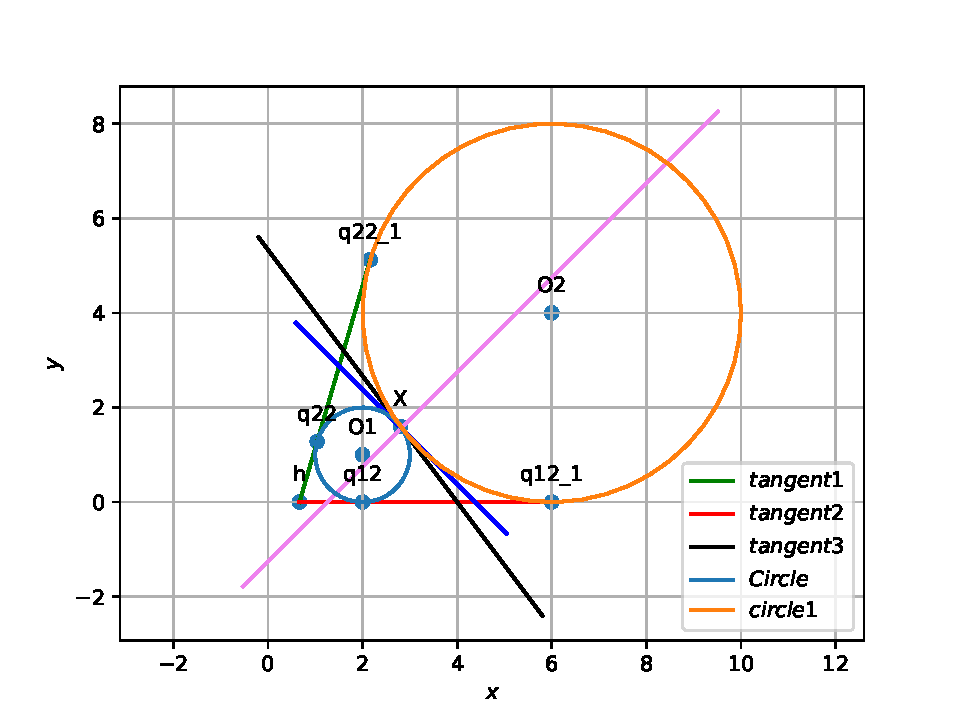
\includegraphics[width=\columnwidth]{fig.pdf}
\caption{Intersection of conics and labeling the common tangents touching the circles in the distinct points.}
		\label{fig:Figure}
\end{figure}
\end{document}